\subsection{PI-controller}

To set the PI-controller the transfer functions for the d- and q-direction is determined, with the voltages as input and the current as output. This is done based on the equations for the voltages in the d- and q-direction, equation \ref{eq:d_direction} and \ref{eq:q_direction}.
Because a transfer function only can have one input and one output, the two equation, \ref{eq:d_direction} and \ref{eq:q_direction}, is shortened. The new equation can be seen in equation \ref{eq:d_direction3} and \ref{eq:q_direction3}.

\begin{equation}
    \label{eq:d_direction3}
    v_d = L_d \frac{d i_d}{dt} + R_s i_d
\end{equation}

\begin{equation}
    \label{eq:q_direction3}
    v_q = L_q \frac{d i_q}{dt} + R_s i_q
\end{equation}

As seen in the two equations, \ref{eq:d_direction3} and \ref{eq:q_direction3}, the parts in the equations depending on other variables than the current is neglected. 
The equations is Laplace transformed and converted to the transfer functions for the two systems.

\begin{equation}
    \label{eq:transfer_d}
    G_d = \frac{I_d(s)}{V_d(s)} = \frac{ \frac{1}{ \frac{L_d}{R_s} } }{ R_s \bigg(\frac{1}{ \frac{L_d}{R_s} } + s \bigg) }
\end{equation}

\begin{equation}
    \label{eq:transfer_q}
    G_q = \frac{I_q(s)}{V_q(s)} = \frac{ \frac{1}{ \frac{L_q}{R_s} } }{ R_s \bigg(\frac{1}{ \frac{L_q}{R_s} } + s \bigg) }
\end{equation}

Equation \ref{eq:transfer_d} and \ref{eq:transfer_q} is the transfer functions for the motor.

To set the PI-controller the cut off frequency is determined. The cut off frequency, $\omega_{cutoff}$, is determined from the time constant of the motor.

\begin{equation}
    \omega_{cutoff} = \frac{1}{\tau}
\end{equation}

$\tau$ is the time constant of motor. The time constant of the motor in the d- and q-direction is described in equation \ref{eq:tau}.

\begin{equation}
    \label{eq:tau}
    \tau_d = \frac{L_d}{R_s}
    , \hspace{1cm}
    \tau_q = \frac{L_q}{R_s}
\end{equation}

From the cut off frequency the cross over frequency is determined.

\begin{equation}
    \label{eq:crossover}
     \omega_c = k_1 \omega_{cutoff}
\end{equation}

Where $k_1$ is a constant which can be changed when tuning the controller.
As the next step the gain margin for the two systems, $G_d$ and $G_q$, multiplied with the transfer function for a PI controller, without the gain. The transfer function for the PI-controller without the gain can be seen in equation \ref{eq:trans_I}.

\begin{equation}
    \label{eq:trans_I}
    G_i = \frac{\tau s + 1}{\tau s}
\end{equation}

The proportional part of the PI-controller is then found from the gain margin, $GM$.

\begin{equation}
    \label{eq:gain}
    K_p = \frac{1}{GM} 
\end{equation}

The $k_1$ is tuned, so that the system gets a phase margin around $70 \degree$. $70 \degree$ phase margin is desired because it results in the fastest response without given any overshoot. At this requirements the $K_p$ is found to be $0.78 \cdot 10^{-3}$ for the d-direction and $0.83 \cdot 10^{-3}$ for the q-direction. The phase margin is $74.1$ for the d-direction and $72.3$ for the q-direction.
A step response for the PI-controller on the motor can be seen figure \ref{fig:step}.

\begin{figure}[H]
	\centering
	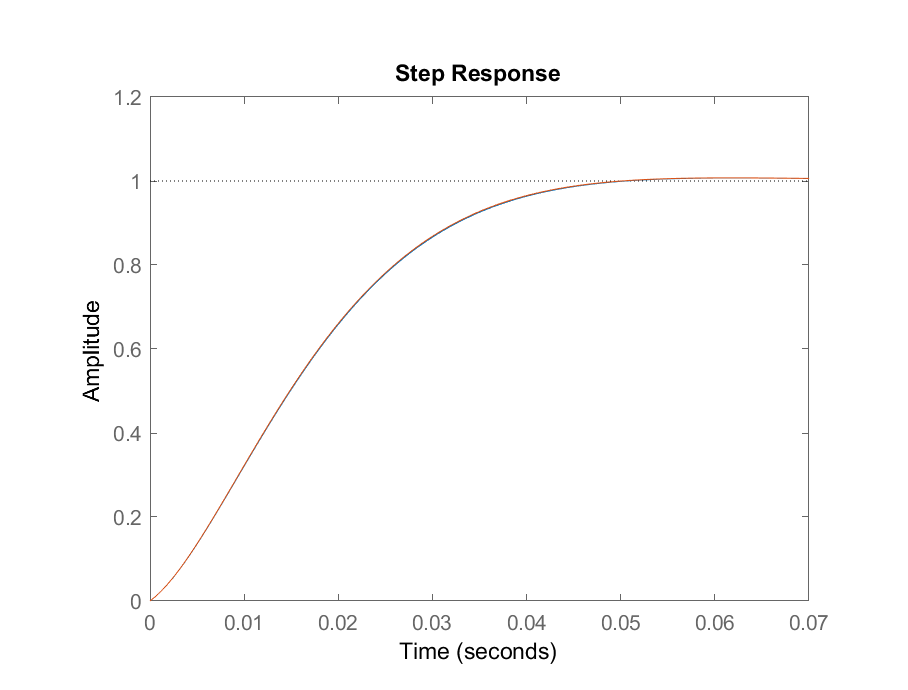
\includegraphics[width=0.6\linewidth]{pictures/control/step_PI.eps}
	\caption{Step response for the controlled motor. The curve for d- and q-direction is placed in top of each other}
	\label{fig:step}
\end{figure}





